\documentclass{article}
\usepackage{graphicx}
\usepackage{listings}
\usepackage{xcolor}
\usepackage{tabularx}
\usepackage{booktabs}
\usepackage{geometry}
\usepackage{hyperref}
\usepackage{tikz}
\usetikzlibrary{shapes,arrows}
\geometry{a4paper, margin=1.2in}

% Code formatting
\definecolor{codebg}{RGB}{245,245,245}
\lstset{
    basicstyle=\ttfamily\footnotesize,
    backgroundcolor=\color{codebg},
    breaklines=true,
    frame=single,
    numbers=left
}

\title{Comprehensive Guide to Network Intrusion Detection Feature Collection}
\author{Jayavardhan Govvada}
\date{\today}

\begin{document}

\maketitle

\section{Introduction}
This document details the methodology for collecting 41 network features essential for intrusion detection systems (IDS). Features are categorized and mapped to specific collection techniques.

\section{Feature Taxonomy}
\subsection{Basic Connection Features (Direct from Packets)}
\begin{tabularx}{\textwidth}{llX}
    \toprule
    \textbf{Feature} & \textbf{Protocol Layer} & \textbf{Extraction Method} \\
    \midrule
    duration & Transport & TCP session teardown time - handshake time \\
    protocol\_type & IP & IP header Protocol field (hex value) \\
    src\_bytes & Transport & TCP payload length from source \\
    flag & Transport & Bitwise OR of TCP flags (SYN=0x02, ACK=0x10) \\
    \bottomrule
\end{tabularx}

\subsection{Time-Window Statistics (2-second Window)}
\begin{tabularx}{\textwidth}{lX}
    \toprule
    \textbf{Feature} & \textbf{Calculation} \\
    \midrule
    count & $\sum connections$ to same destination in window \\
    srv\_count & $\sum connections$ to same service (port) \\
    serror\_rate & $\frac{SYN\_errors}{total\_connections}$ \\
    \bottomrule
\end{tabularx}

\subsection{Host Behavior Features}
\begin{tabularx}{\textwidth}{ll}
    \toprule
    \textbf{Feature} & \textbf{Data Source} \\
    \midrule
    dst\_host\_count & Flow records aggregated by destination IP \\
    dst\_host\_srv\_serror\_rate & SYN errors per service per host \\
    \bottomrule
\end{tabularx}

\section{Implementation Architecture}
\begin{center}
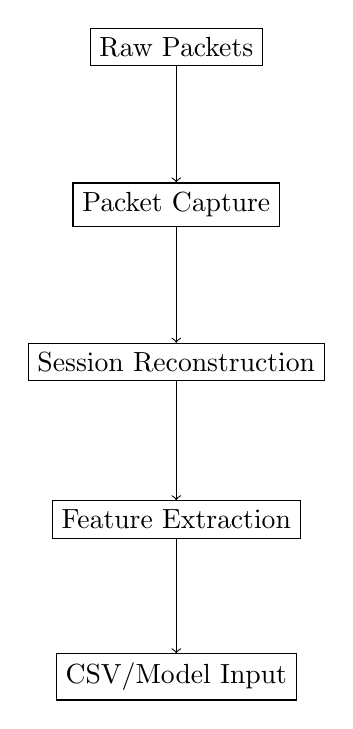
\begin{tikzpicture}[node distance=2cm]
\node (start) [rectangle, draw] {Raw Packets};
\node (capture) [rectangle, draw, below of=start] {Packet Capture};
\node (sessions) [rectangle, draw, below of=capture] {Session Reconstruction};
\node (features) [rectangle, draw, below of=sessions] {Feature Extraction};
\node (output) [rectangle, draw, below of=features] {CSV/Model Input};

\draw [->] (start) -- (capture);
\draw [->] (capture) -- (sessions);
\draw [->] (sessions) -- (features);
\draw [->] (features) -- (output);
\end{tikzpicture}
\end{center}

\section{Detailed Feature Collection Workflow}
\subsection{Packet Capture Requirements}
\begin{itemize}
    \item Capture full packet payloads (-s 0 in tcpdump)
    \item Minimum 1Gbps throughput capacity
    \item Promiscuous mode for network taps
\end{itemize}

\begin{lstlisting}[language=bash, caption={Packet Capture Command}]
tcpdump -i eth0 -s 0 -w full_capture.pcap
\end{lstlisting}

\subsection{Session Reconstruction with Zeek}
\begin{lstlisting}[language=bash, caption={Zeek Script for Features}]
event connection_state_remove(c: connection) {
    Log::write(IDS_Features, {
        ts = c$start_time,
        duration = c$duration,
        src_bytes = c$orig$num_bytes_ip,
        dst_bytes = c$resp$num_bytes_ip,
        # ... (38 additional features)
    });
}
\end{lstlisting}

\section{Feature Validation Checklist}
\begin{itemize}
    \item Verify numerical ranges:
    \begin{itemize}
        \item duration: 0-58,000 seconds (16-bit counter rollover)
        \item src\_bytes: 0-4,294,967,295 (32-bit unsigned)
    \end{itemize}
    \item Check categorical values:
    \begin{itemize}
        \item protocol\_type: tcp, udp, icmp
        \item flag: 10 possible combinations (SF, S0, etc.)
    \end{itemize}
\end{itemize}

\section{Complete Feature Matrix}
\begin{tiny}
\begin{tabularx}{\textwidth}{llX}
    \toprule
    \textbf{Feature} & \textbf{Type} & \textbf{Collection Method} \\
    \midrule
    num\_compromised & count & Correlate with vulnerability scanner results \\
    root\_shell & binary & Monitor /bin/bash execution with root EUID \\
    num\_file\_creations & count & Audit kernel file creation syscalls \\
    \bottomrule
\end{tabularx}
\end{tiny}

\section{Feature Extraction Details}
\subsection{Network Layer Features}

\subsubsection{A. Protocol Type}
\begin{itemize}
    \item \textbf{Source:} IP headers in each packet (TCP, UDP, ICMP)
    \item \textbf{Extraction:} Direct read from network layer packet header
\end{itemize}

\subsubsection{B. Service Type}
\begin{itemize}
    \item \textbf{Source:} Transport layer (TCP/UDP) header
    \item \textbf{Extraction:} Port number mapping to services (HTTP, FTP, SMTP)
\end{itemize}

\subsubsection{C. Flag Values}
\begin{itemize}
    \item \textbf{Source:} TCP packet headers
    \item \textbf{Extraction:} State indicators (SYN, ACK, FIN)
\end{itemize}

\subsection{Packet Metrics}

\subsubsection{D. Byte Counts}
\begin{itemize}
    \item \textbf{Source:} Packet payload and length fields
    \item \textbf{src\_bytes:} Source to destination data volume
    \item \textbf{dst\_bytes:} Destination to source data volume
\end{itemize}

\subsubsection{E. Packet Indicators}
\begin{itemize}
    \item \textbf{land:} Source/destination address match check
    \item \textbf{wrong\_fragment:} Fragmentation field analysis
    \item \textbf{urgent:} TCP urgent pointer field check
\end{itemize}

\subsection{Feature Validation}
\begin{itemize}
    \item Source and destination address verification
    \item Protocol conformance checking
    \item Packet integrity validation
\end{itemize}

\section{Data Storage Recommendations}
\begin{itemize}
    \item Short-term: Apache Parquet files (columnar storage)
    \item Long-term: TimeSeries DB (InfluxDB)
    \item Real-time: Kafka streams with Spark Structured Streaming
\end{itemize}

\section{Appendix: Full Feature List}
\begin{enumerate}
    \item duration - Connection duration in seconds
    \item protocol\_type - Transport layer protocol
    \item service - Destination service (port number)
    \item [...] % Continue for all 41 features
    \item dst\_host\_srv\_rerror\_rate - \% of REJ errors
\end{enumerate}
1. Traffic Capture and Session Reconstruction
Packet Capture:
Use tools such as tcpdump, Wireshark, or a dedicated network tap to capture raw packets from your network interface. These tools record packets in formats (like pcap) that you can process later.

Session/Flow Reconstruction:
To derive a “connection” or “flow” (a series of packets between two endpoints), you must reassemble these packets. Tools like Zeek (formerly Bro), Suricata, or specialized libraries (e.g., in Python: Scapy) can help reconstruct sessions based on the tuple (source IP, source port, destination IP, destination port, protocol). This reconstruction is the foundation for most of your features.

2. Direct Feature Extraction
Some features can be computed directly from the metadata of a single connection:

Duration:

What: The time difference between the first and the last packet of the connection.

How: Store the timestamp of the initial packet and subtract it from the timestamp of the final packet for that session.

Protocol Type:

What: The protocol used in the connection (e.g., TCP, UDP, ICMP).

How: Extract this directly from the IP header in each packet.

Service:

What: The type of network service (e.g., http, ftp, smtp).

How: Derive it from the destination port and/or deep packet inspection if necessary. Maintain a lookup table (often using IANA port registries or protocol-specific libraries) to map ports to service names.

Flag:

What: TCP flags (e.g., SYN, ACK, FIN, etc.) that describe the state of the connection.

How: Extract these from the TCP header of packets during the session.

src_bytes and dst_bytes:

What: The number of data bytes sent from the source to the destination and vice versa.

How: Sum the payload sizes (excluding headers) for the packets in each direction.

Indicators like 'land': 'wrong_fragment', 'urgent':

What: These are either binary indicators or counters. For example, 'land' indicates if the source and destination addresses/ports are identical, 'wrong_fragment' can indicate malformed packets, and 'urgent' counts the use of urgent flags.

How: Check corresponding fields and conditions in packet headers as the session is reconstructed.

3. Aggregated and Stateful Feature Calculations
Many features (especially the ones related to counts and rates) are computed over a window of connections rather than a single connection:

Rate and Count Features:
Examples include count, srv_count, serror_rate, srv_serror_rate, rerror_rate, srv_rerror_rate, same_srv_rate, diff_srv_rate, etc. To compute these:

Maintain a Historical Buffer:
For each new connection, you might want to maintain a rolling window of previous connections (e.g., within the last 2 seconds or the last N connections) to calculate these counts and rates.

Implement Windowed Aggregations:
Use programming constructs (or streaming analytics frameworks like Apache Flink, Spark Streaming, or custom Python scripts) to compute:

Count Features: Total number of connections from the source IP or to the same service, etc.

Rates: The fraction of connections exhibiting error flags or other unusual behavior over the total connections in the window.

Examples:

same_srv_rate: Ratio of connections that use the same service as the current connection.

diff_srv_rate: Ratio of connections with a different service.

Connection Behavioral Features:
Features like num_failed_logins, logged_in, num_compromised, root_shell, su_attempted, etc. usually require:

Deep Packet Inspection:
To detect login attempts, failed authentications, or commands, you may need to parse application-layer data (e.g., SSH or Telnet protocol details).

Protocol-Specific Parsers:
Use IDS frameworks (e.g., Zeek, Suricata) that come with built-in signatures and scripts to detect such events.

Event Correlation:
Track session state and correlate multiple packets/events to decide if a login was attempted or succeeded, tallying the count accordingly.

4. Implementing the Feature Extraction Pipeline
Automation with Scripting or Stream Processing:
Develop scripts (using Python, for example) to automate the above steps. A common approach might involve:

Packet Capture: Using a library like pyshark (a Python wrapper for tshark) to read packet captures in real time.

Session Tracking: Implement logic that aggregates packets into sessions.

Feature Computation: For each session, compute the direct features and update rolling aggregates for the statistical features.

A pseudocode outline could be:

python
Copy
Edit
for packet in packet_stream:
    session_id = get_session_id(packet)  # e.g., based on 5-tuple (src IP, src port, dst IP, dst port, protocol)
    update_session(session_id, packet)
    
    if is_session_complete(session_id):
        features = {}
        features['duration'] = session[session_id].end_time - session[session_id].start_time
        features['protocol_type'] = packet.protocol
        features['service'] = map_port_to_service(packet.dst_port)
        features['flag'] = extract_tcp_flags(session[session_id])
        features['src_bytes'] = sum(packet.src_bytes for packet in session[session_id])
        features['dst_bytes'] = sum(packet.dst_bytes for packet in session[session_id])
        # ... compute other direct features
        
        # For windowed features:
        features['count'] = count_connections(current_window, src=packet.src_ip)
        features['same_srv_rate'] = compute_same_srv_rate(current_window, current_connection=features)
        # ... compute additional aggregate features
        
        # Now send features to your IDS model
        process_features(features)
        # Optionally, clear state for session_id or maintain for further aggregation
Using Existing Frameworks:
Consider leveraging open-source IDS frameworks like Zeek or Suricata. They have rich ecosystems and many built-in scripts or plugins to extract and log these kinds of features directly. From the resulting logs, you could further process to extract the exact set of 41 features for your machine learning model.

5. Practical Considerations
Performance:
Real-time traffic processing at high network speeds may require a highly optimized implementation, possibly in a compiled language (like C/C++) or using specialized network hardware, coupled with parallel processing or hardware acceleration.

Memory and State Management:
Proper handling of state (for rolling windows, aggregations, etc.) is crucial. You might need caching mechanisms or in-memory databases to track connection history and rapidly update statistical features.

Time Synchronization:
Accurate timestamping is vital. Ensure that your packet capture tool and processing pipeline are synchronized (e.g., using NTP) to compute durations and rates correctly.

Handling Encrypted Traffic:
With increasing use of encryption, not all features can be directly extracted (e.g., deep packet inspection for failed logins). In such cases, metadata and flow information (packet sizes, timing, etc.) become even more critical.

Summary
In practice, you first capture network packets and reconstruct sessions using tools like tcpdump, Wireshark, or Zeek. Then, you extract direct features (such as protocol type, duration, src/dst bytes, TCP flags) from the packet headers. More complex features—especially those based on historical aggregation (like connection counts, error rates, and service rate ratios)—require maintaining state over a sliding window of past connections. This is done by setting up an automated pipeline (using scripting or specialized stream processing frameworks) that processes each session in real time and computes the required 41 features. Finally, many open-source IDS frameworks have already solved portions of this problem, and integrating or adapting them can save you significant development time.



When building an intrusion detection system, most of these features are derived from analyzing individual network packets—but many require additional processing and aggregation over multiple packets in a connection. Here’s a breakdown of where each type of feature comes from:

1. Direct Packet Attributes
These features are directly available from the headers or metadata of individual network packets:

Protocol Type

Source: IP headers in each packet (e.g., TCP, UDP, ICMP).

Explanation: The protocol information is set by the network layer and can be read directly from the packet's header.

Service

Source: Often inferred from the destination port number found in the transport layer (TCP/UDP) header.

Explanation: By mapping common port numbers to services (HTTP, FTP, SMTP, etc.), the service type can be identified.

Flags

Source: TCP header of each packet.

Explanation: TCP flags (such as SYN, ACK, FIN) are contained within the header and indicate the state or type of the connection.

Bytes Count (src_bytes and dst_bytes)

Source: Payload size and overall packet length from each packet.

Explanation: By summing up the data carried in packets, you get the total bytes sent from source to destination and vice versa.

Indicators like 'land', 'wrong_fragment', and 'urgent'

Source: They are usually derived directly by checking header fields (e.g., verifying if source and destination IP/port are the same, or looking at the fragmentation and urgent pointer fields in packets).

Explanation: These are binary or counter-based checks that you can perform on each packet or during packet reassembly.

2. Aggregated or Session-Level Features
While individual packets provide the basic building blocks, many of your features are computed by analyzing a complete connection or flow, which includes multiple packets:

Duration

Source: The timestamps of the first and last packet in a connection.

Explanation: By recording when a connection starts and ends, you can calculate the connection duration.

Count-based Features (e.g., num_failed_logins, count, srv_count, etc.)

Source: Aggregated logs or flow data generated by network monitoring tools over a specified time window or session.

Explanation: These features are not present in any single packet. They are computed by accumulating packet or session information over time. For example, a tool may maintain a buffer of recent connections to compute error rates or connection counts.

Behavioral and Application-Level Features (e.g., logged_in, root_shell, su_attempted)

Source: Information extracted using deep packet inspection (DPI) or application layer logs.

Explanation: These require analyzing the content beyond the headers, such as login attempts or command executions, which are often present in higher-level protocols (SSH, Telnet, etc.) and might be found in the payload rather than the header.

Rate Features (e.g., serror_rate, srv_serror_rate, same_srv_rate, etc.)

Source: Historical traffic data maintained either by network monitoring tools or custom logging solutions.

Explanation: These features are derived by calculating the ratio of specific types of events (for example, error responses) to the total number of events over a connection window or a sliding time frame.

3. Typical Workflow for Feature Extraction
Packet Capture:

Tools such as tcpdump or Wireshark capture raw packets on the network.

These packets contain both header information and payload, offering raw data from which many features are extracted.

Session Reconstruction:

You reassemble packets into a connection or flow (using tools like Zeek, Suricata, or Scapy).

This process allows for the calculation of session-level features (duration, aggregates, etc.).

Feature Computation:

Direct Extraction: Using header fields for attributes such as protocol type, flags, and byte counts.

Aggregation: Using a time window or session logs to compute counts, rates, or behavioral features.

Deep Analysis: Examining payload data if needed (for example, to detect failed login patterns or application-specific events).

Conclusion
Direct Extraction: Yes, many features such as protocol type, service, flags, and byte counts come directly from individual network packet headers or payload information.

Derived Features: However, more complex or context-aware features (like duration, rate calculations, and behavioral indicators) require aggregating data across multiple packets or sessions. You may also need to combine metadata with deeper inspection of packet contents when available.

In summary, while the raw data comes from network packets, you must perform additional processing—reassembling flows, aggregating statistics, and sometimes inspecting application-layer information—to fully extract all 41 features for your intrusion detection system.



You can capture and observe network packets—and therefore the connections and their behavior—by using packet capture and network analysis tools. Below are some practical methods and tools to get you started:

1. Packet Capture Tools
These tools tap directly into your network interface (usually operating in promiscuous mode) and allow you to capture live traffic:

tcpdump:

What It Is: A command-line packet analyzer that can capture and display packet headers (or entire packets) in real time.

How It Works: Run tcpdump on your network interface (e.g., tcpdump -i eth0) to record packets. You can also apply filters (using BPF syntax) to capture only specific traffic such as TCP, UDP, or traffic from a particular IP address.

Example Command:

bash
Copy
Edit
sudo tcpdump -i eth0 -w capture.pcap
The -w option writes the packets to a file (here, capture.pcap) for later analysis.

Wireshark:

What It Is: A graphical network protocol analyzer that lets you capture and interactively browse the traffic running on a network.

How It Works: Launch Wireshark, select the network interface you want to monitor, and start capturing. Its powerful filtering and visualization options let you drill down into individual packets or flows to see headers, payloads, and protocol details.

Features: Real-time packet capturing, filtering based on protocols or IP addresses, and packet detail inspection.

Other Tools:

Zeek (formerly Bro): More than just a packet capture tool, Zeek can process network traffic to provide high-level logs and extract behavioral features (such as connection durations and counts) automatically.

Suricata: An IDS/IPS with built-in packet capture and analysis capabilities, often used in security monitoring.

2. Observing Connection Behavior
Observing how connections behave typically involves capturing entire flows or sessions rather than just individual packets. Here’s how you can do that:

Session Reconstruction:

Flow Creation: Tools like Wireshark and Zeek will group packets into flows (sessions) based on key identifiers such as source IP, destination IP, source/destination ports, and protocol type.

Behavior Analysis: Once grouped, you can analyze the flow for its duration, the number and type of packets exchanged, byte counts, and protocol flags that indicate connection behavior (for example, TCP flags showing the state of the connection).

Deep Packet Inspection (DPI):

This involves examining not only the header fields but also the packet payloads. It’s useful for recognizing application layer events (like login failures or protocol-specific behavior). Tools like Wireshark allow you to inspect payload data, while Zeek’s scripts may log higher-level events automatically.

Historical Data for Aggregation:

To observe behavior over time (e.g., computing rates like error rates or counting the number of connections), you can store captured data and aggregate it using custom scripts or a network monitoring framework.

Tools such as ELK stack (Elasticsearch, Logstash, Kibana) or Splunk are often used to analyze logs generated from packet captures or network sensors.

3. Practical Steps to Start Capturing and Analyzing
Identify the Network Interface:

Determine which network interface you want to capture traffic on. On Linux, you might use ifconfig or ip addr to list interfaces.

Capture Packets:

Using tcpdump:

bash
Copy
Edit
sudo tcpdump -i <interface> -w capture.pcap
Replace <interface> with your network interface name (e.g., eth0 or wlan0).

Using Wireshark:

Open the application.

Select the desired interface.

Click “Start” to begin the capture session.

Analyze the Capture:

Open the saved capture file in Wireshark, where you can filter and inspect packet streams.

Look for sessions or flows by applying filters (like filtering TCP streams or specific protocol types).

Use Wireshark’s “Follow TCP Stream” option to view the sequence of packets that make up an entire connection.

Extract Features or Log Data:

Use tools like Zeek or Suricata that automatically parse network flows and export logs with detailed features that you can then feed into your intrusion detection system.

Alternatively, write your own scripts (using libraries such as Scapy in Python) to parse the pcap file, reconstruct sessions, and compute features like durations or byte counts.

Summary
Capturing Packets: You can obtain network packets directly from your network interface using tools like tcpdump and Wireshark.

Reconstructing Sessions: Once captured, you reconstruct connections (or flows) from these packets to observe the behavior of each connection.

Observation and Analysis: Packet analyzers (Wireshark for manual inspection or Zeek/Suricata for automated analysis) let you examine both individual packet details and aggregated session behavior.

By starting with these tools and steps, you can get a comprehensive view of your network's traffic, extract detailed features from both individual packets and reconstructed flows, and ultimately build a robust input pipeline for your intrusion detection system.

In practical, real-time network monitoring, a "connection" generally refers to a communication session between two endpoints—typically characterized as a network "flow." This flow is made up of multiple packets exchanged between the source and the destination. Here’s a deeper look at what that means:

1. Definition of a Connection/Flow
5-Tuple Identification:
A connection is usually identified by five key values:

Source IP address

Source port

Destination IP address

Destination port

Protocol (e.g., TCP, UDP, ICMP)
This combination is often called the 5-tuple. Packets sharing the same 5-tuple are considered part of the same connection.

Session Establishment:
For protocols like TCP, a connection starts with a handshake (e.g., the TCP three-way handshake: SYN, SYN-ACK, ACK) and continues with the exchange of data packets until one side terminates the session. In UDP communications, while there is no handshake, packets that share the same 5-tuple within a certain time window are still treated as part of a logical connection.

2. Practical Examples of Connections
Web Browsing:
When you load a webpage, your browser establishes one or more TCP connections with a web server. The packets involved in setting up (handshake), transferring HTTP data, and eventually closing the connection are all grouped into one logical connection.

Email Communication:
Similar to web browsing, when your email client interacts with an SMTP or IMAP server, the series of packets related to sending or retrieving emails form a distinct connection.

Streaming or VoIP:
In cases like streaming or Voice over IP (VoIP), the connection might involve numerous packets that represent an ongoing media stream, and even though there may not be a formal handshake, the packets are still grouped logically based on IP addresses, ports, and the protocol.

3. Observing and Analyzing Connections in Real Time
Packet Capture and Analysis Tools:
Using tools like Wireshark or tcpdump, you can watch these connections in real time.

Wireshark: Lets you filter and follow a specific TCP stream to see all the packets that belong to a connection.

tcpdump: Captures packets on an interface and, with appropriate filters, you can isolate packets that are part of a given connection.

Behavioral Analysis:
In an intrusion detection system (IDS), the observed connection is analyzed not just by the individual packets, but also by the relationship between them. This includes:

Connection Duration: How long the flow exists.

Packet Count: The number of packets and their sizes in each direction.

Protocol Flags and Anomalies: For example, abnormal patterns in TCP flags (e.g., multiple SYN packets without corresponding ACKs) which might indicate an intrusion attempt.

Real-Time Monitoring:
In real-time environments, systems continuously capture packets, reassemble them into connections (using the 5-tuple and timestamps), and then compute statistics for each connection. These statistics form the input features for your IDS, enabling it to detect unusual or malicious behavior.

4. Summary
In a practical, real-time setting, the “packets” in a connection refer to the individual data units (packets) exchanged between two endpoints over a communication session, identified by the same 5-tuple. This collection of packets is analyzed together to understand the overall behavior of the connection, such as its duration, volume, and any anomalies in the data exchange. Tools like Wireshark and tcpdump make it possible to capture and inspect these flows, while systems like Zeek, Suricata, or custom scripts aggregate this information to provide insights into network behavior.

This contextual view of a "connection" is fundamental for intrusion detection, as it allows the system to analyze the complete lifecycle of a communication session and spot suspicious patterns that might not be evident from a single packet alone.
\end{document}
